Table~\ref{tab:capacity} states, for every state and party, the number of districts that can simultaneously reach 50\%, 55\% and 60\% of the two-party vote; a single number is an exact value of $F_\rho(m)$ (certified lower and upper bounds coincide) and an interval $a$--$b$ gives $a\le F_\rho(m)\le b$. Figure~\ref{fig:frontier2} shows the certified frontiers of the six two-district states with the region between the certified lower and upper staircases shaded (invisible when the bracket is a fraction of a point wide), Figure~\ref{fig:frontier3} those of the states with $3\le k\le5$, and Table~\ref{tab:spectrum} in the appendix lists every bracket for $\sigma^*(q)$.

\begin{table}[!tbp]
\centering\small
\caption{Certified seat--safety capacity at $\rho_s$ ($\pm1\%$, $k-1$ county splits, 2020 presidential two-party vote): number of districts that can simultaneously have at least the stated party share. Single number = exact; $a$--$b$ = certified interval.}\label{tab:capacity}
\adjustbox{max width=\linewidth}{\begin{tabular}{llrcccc}
\toprule
State & Party & $k$ & stat.\ share & $\ge50\%$ & $\ge55\%$ & $\ge60\%$ \\
\midrule
New Hampshire & D & 2 & 53.7\% & 2 & 1 & 0 \\
New Hampshire & R & 2 & 46.3\% & 0 & 0 & 0 \\
Maine & D & 2 & 54.7\% & 2 & 1 & 1 \\
Maine & R & 2 & 45.3\% & 1 & 0 & 0 \\
Rhode Island & D & 2 & 60.6\% & 2 & 2 & 2 \\
Rhode Island & R & 2 & 39.4\% & 0 & 0 & 0 \\
Idaho & D & 2 & 34.1\% & 0 & 0 & 0 \\
Idaho & R & 2 & 65.9\% & 2 & 2 & 2 \\
Montana & D & 2 & 41.6\% & 1 & 0 & 0 \\
Montana & R & 2 & 58.4\% & 2 & 2 & 1 \\
West Virginia & D & 2 & 30.2\% & 0 & 0 & 0 \\
West Virginia & R & 2 & 69.8\% & 2 & 2 & 2 \\
Nebraska & D & 3 & 40.2\% & 1--2 & 1 & 0--1 \\
Nebraska & R & 3 & 59.8\% & 3 & 3 & 2 \\
New Mexico & D & 3 & 55.5\% & 3 & 3 & 2 \\
New Mexico & R & 3 & 44.5\% & 2 & 1 & 1 \\
Arkansas & D & 4 & 35.8\% & 1--2 & 1 & 0--1 \\
Arkansas & R & 4 & 64.2\% & 4 & 4 & 4 \\
Iowa & D & 4 & 45.8\% & 3 & 2 & 1 \\
Iowa & R & 4 & 54.2\% & 4 & 3 & 2--3 \\
Kansas & D & 4 & 42.5\% & 2--3 & 1--2 & 1 \\
Kansas & R & 4 & 57.5\% & 4 & 3--4 & 3 \\
Mississippi & D & 4 & 41.6\% & 2--3 & 1--2 & 1--2 \\
Mississippi & R & 4 & 58.4\% & 4 & 4 & 3 \\
Nevada & D & 4 & 51.2\% & 3--4 & 2 & 2 \\
Nevada & R & 4 & 48.8\% & 3 & 2 & 0--1 \\
Utah & D & 4 & 39.3\% & 2 & 1 & 1 \\
Utah & R & 4 & 60.7\% & 4 & 4 & 3--4 \\
Connecticut & D & 5 & 60.2\% & 5 & 5 & 5 \\
Connecticut & R & 5 & 39.8\% & 1 & 0 & 0 \\
Oklahoma & D & 5 & 33.1\% & 1--2 & 0--1 & 0--1 \\
Oklahoma & R & 5 & 66.9\% & 5 & 5 & 5 \\
\bottomrule
\end{tabular}
}
\end{table}

\begin{figure}[!tbp]
\centering
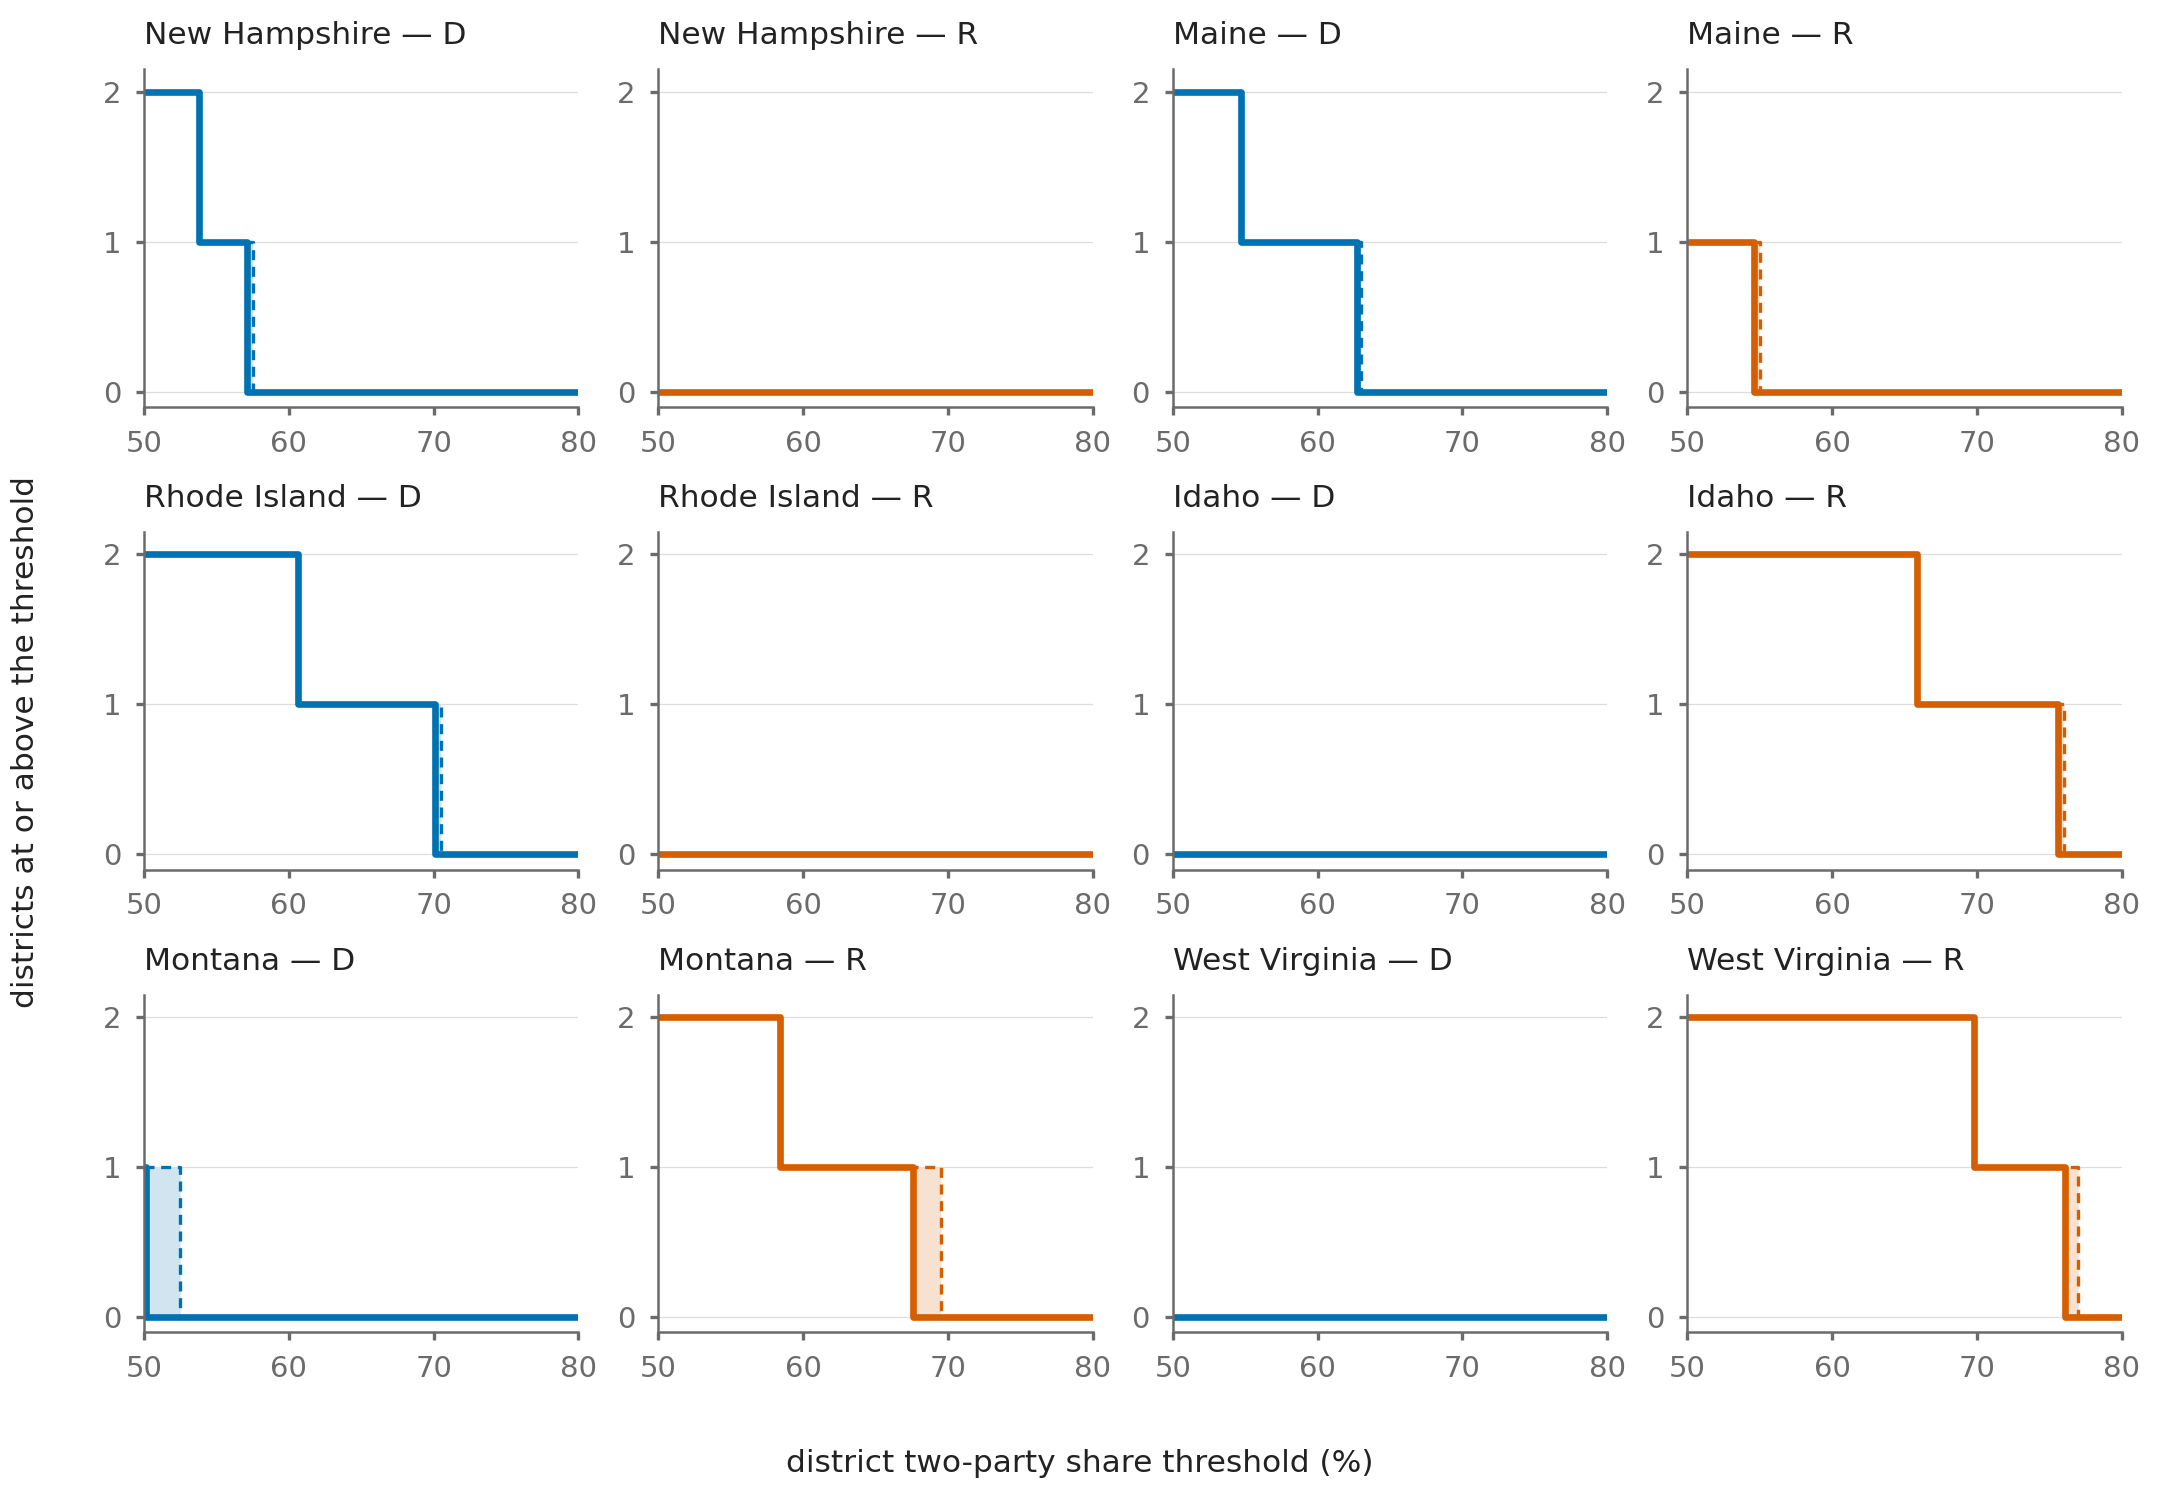
\includegraphics[width=\linewidth]{figs/frontier_k2.png}
\caption{Certified seat--safety frontiers $F(m)$ for the two-district states, both parties. Solid: certified lower staircase (independently verified plans); dashed: certified upper staircase (infeasibility proofs); shading: unresolved band. A party with no line above zero cannot make a district of that share in any plan of the regime.}\label{fig:frontier2}
\end{figure}

\paragraph{Exactness.}
At the three thresholds of Table~\ref{tab:capacity}, 79 of the 96 values of $F$ are pinned exactly: all 36 in the two-district states and 43 of the 60 in the states with three to five districts. Over a one-point grid of thresholds from 50\% to 80\%, 80\% of the 992 (state, party, threshold) values are exact. In terms of the spectrum (Table~\ref{tab:tightness}), 21 of the 24 brackets in the two-district states are tight to half a point of district share (median width 0.01 point once the geography-free bound is used as an additional upper bound) and the median bracket for $3\le k\le5$ is 2.2--2.6 points wide; the widest open brackets (9--14 points) are those of a party that is a minority in a state with three or more districts (Mississippi and Arkansas Democrats at $q=2$, Connecticut Democrats at $q=1$, Mississippi Republicans at $q=2$, Oklahoma Democrats).

\begin{table}[!tbp]
\centering\small
\caption{Width of the certified brackets $[r_q,u_q)$ for $\sigma^*(q)$, in points of district share, by number of districts $k$. Brackets proving that no $q$ districts can reach 50\% count as exact.}\label{tab:tightness}
\adjustbox{max width=\linewidth}{\begin{tabular}{crrrrrr}
\toprule
$k$ & brackets & exact ($\le0.5$ pt) & $\le1$ pt & $\le2$ pt & $\le3$ pt & median width (pts) \\
\midrule
2 & 24 & 21 & 22 & 23 & 24 & 0.01 \\
3 & 12 & 4 & 5 & 6 & 9 & 2.23 \\
4 & 48 & 10 & 12 & 19 & 27 & 2.62 \\
5 & 20 & 9 & 9 & 10 & 13 & 2.21 \\
\bottomrule
\end{tabular}
}
\end{table}

\paragraph{What the exact values say.}
(i) \emph{Certified zeros.} Republicans in New Hampshire and Rhode Island and Democrats in Idaho and West Virginia provably cannot make even one majority district (for Rhode Island, Idaho and West Virginia the geography-free bound already shows it; for New Hampshire Republicans it needs geography: the hull bound allows up to 54.6\%). (ii) \emph{Packing gains.} The best single district of a party can be far above the party's statewide share (Figure~\ref{fig:scatter}): for example Idaho Republicans (65.9\% statewide) can reach 75.5--76.0\%, Rhode Island Democrats (60.6\%) 70.0--70.5\%, and Maine Democrats (54.7\%) 62.7--63.0\% (Figure~\ref{fig:maps} shows witness plans for three of these states). (iii) \emph{The all-safe end is pinned by the statewide share.} Because the turnout-weighted mean of the district margins equals the statewide margin, $\sigma^*(k)$ cannot exceed it, and the resolved certified values sit within 0.2 point of it (Idaho Republicans $q=2$: 65.88\% against 65.9\%; Nebraska Republicans $q=3$: 59.71\% against 59.8\%; Connecticut Democrats $q=5$: 60.12\% against 60.2\%). (iv) \emph{A one-seat statement with geography.} Connecticut Republicans (39.8\% statewide) can make exactly one district with at least 50\%, and none with at least 55\%.

\begin{figure}[!tbp]
\centering
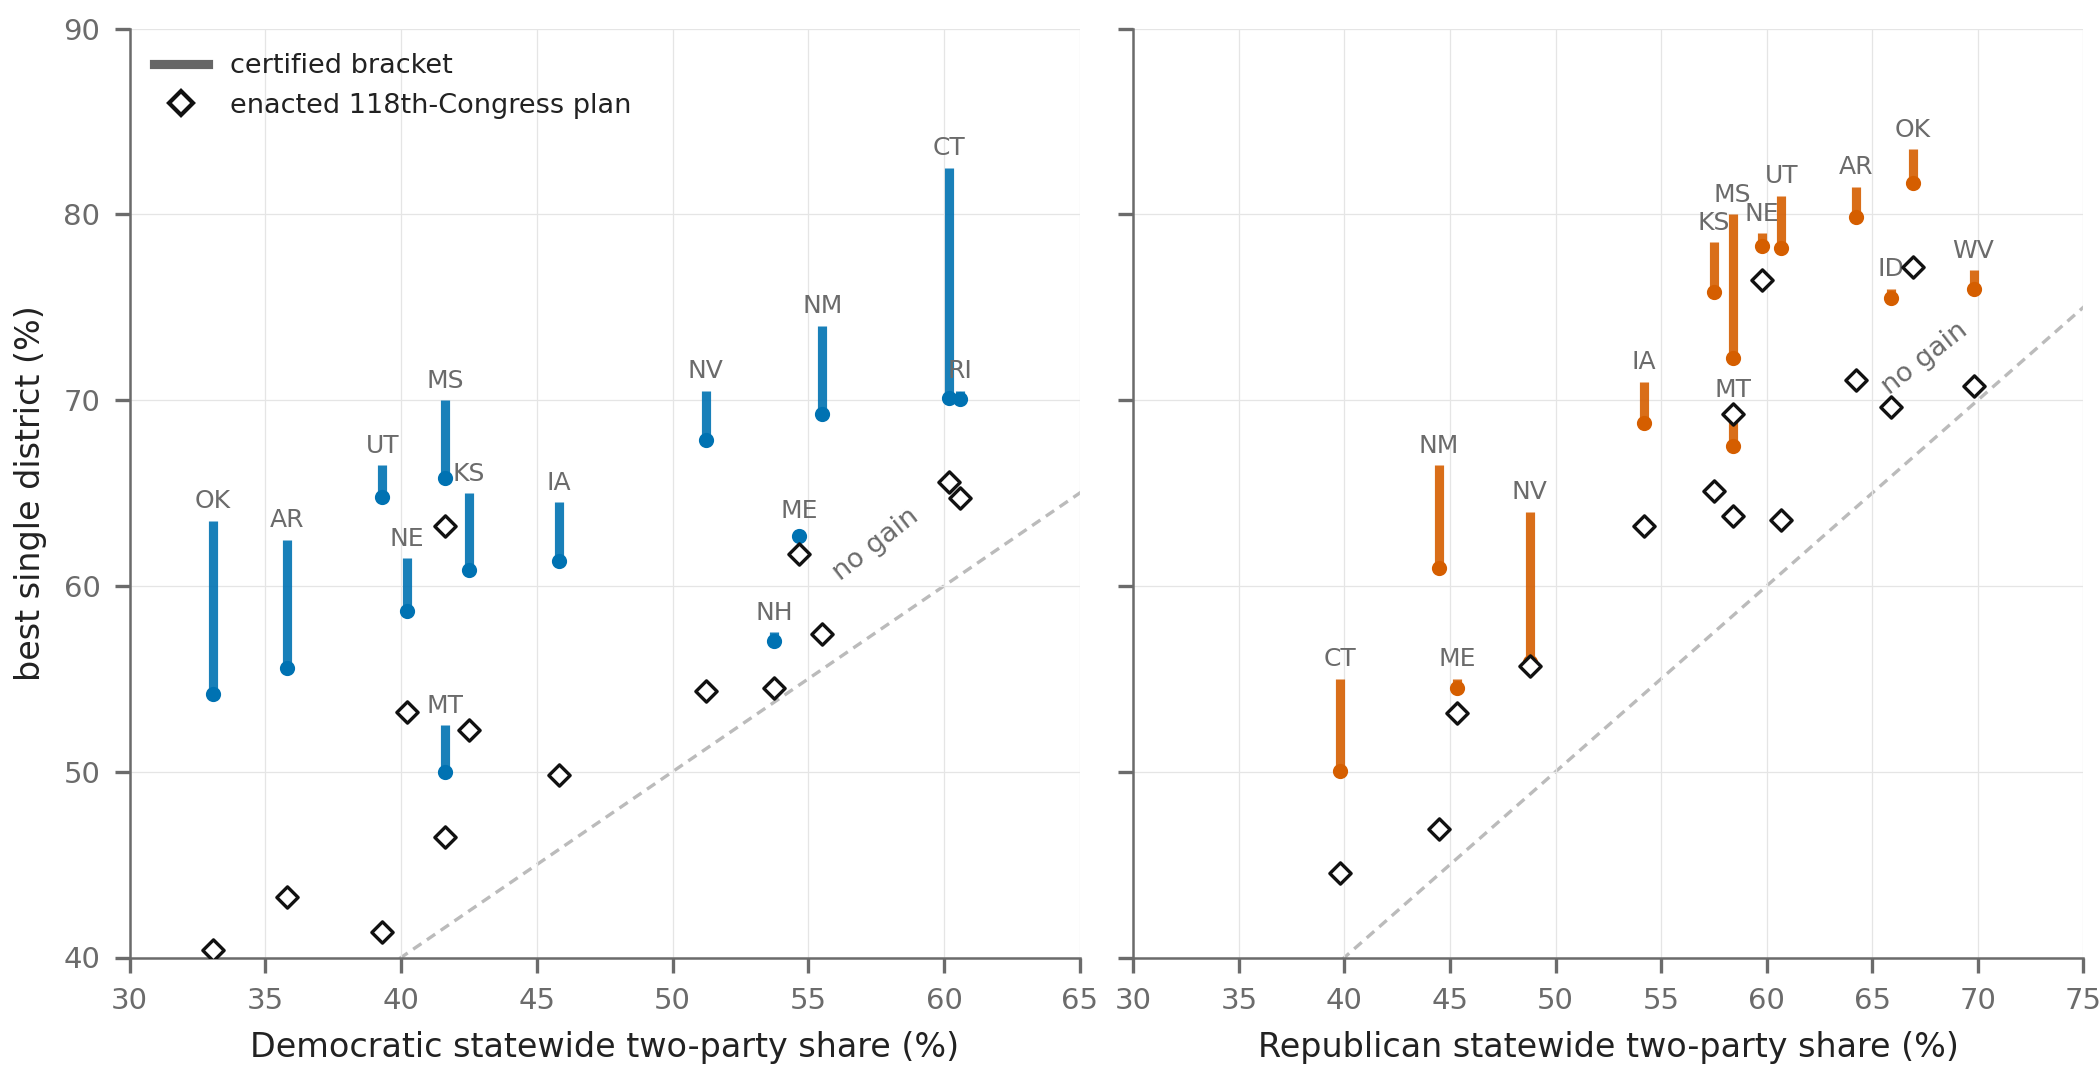
\includegraphics[width=\linewidth]{figs/scatter.png}
\caption{Certified bracket for the best single district ($q=1$) against the party's statewide two-party share. Points on the dashed diagonal would mean the boundaries give no gain.}\label{fig:scatter}
\end{figure}

\begin{figure}[!tbp]
\centering
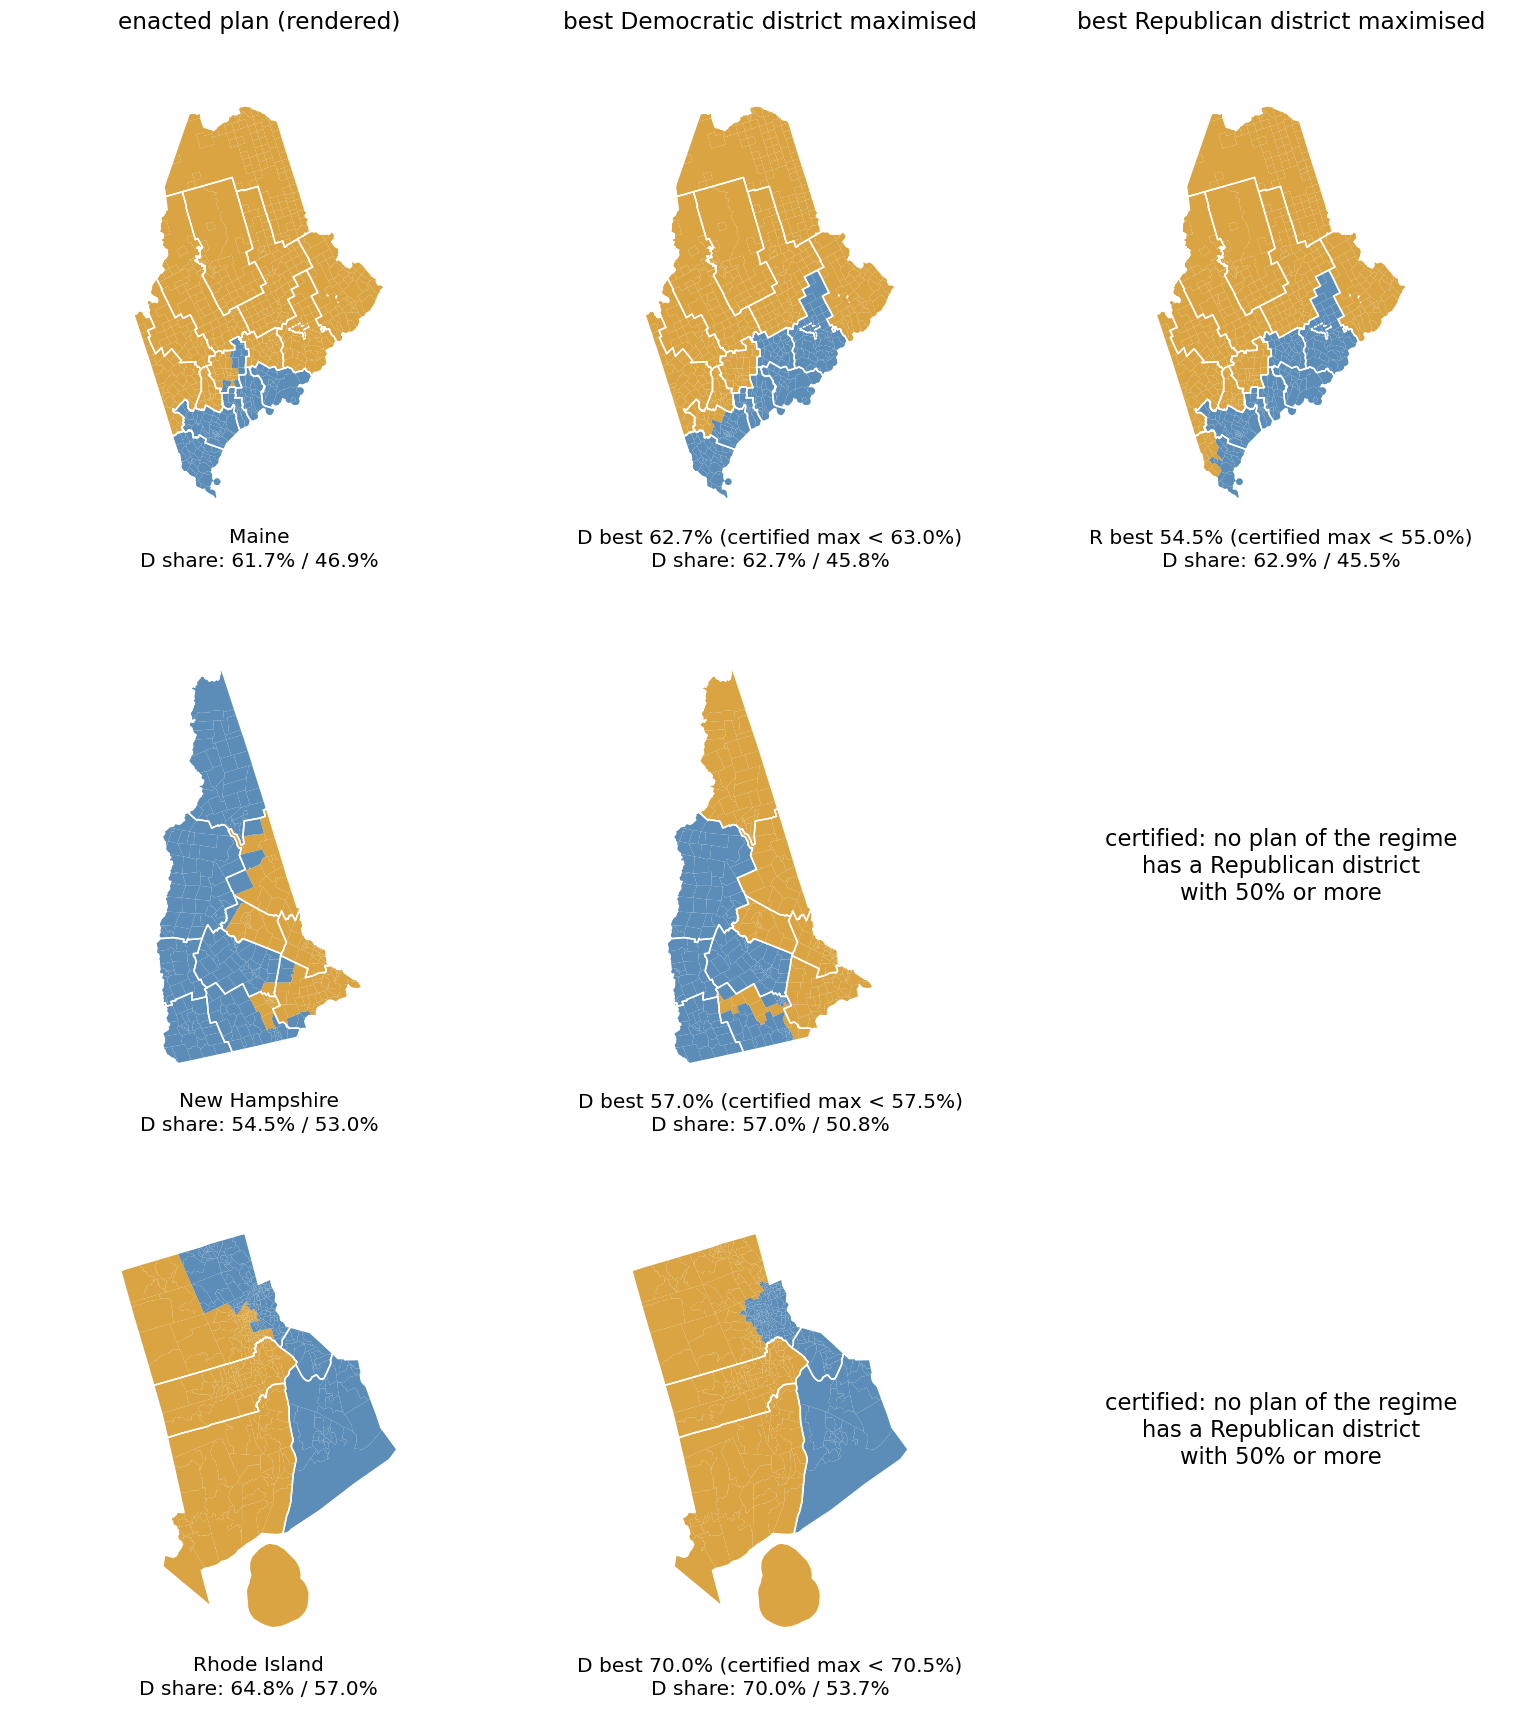
\includegraphics[width=0.9\linewidth,height=0.74\textheight,keepaspectratio]{figs/maps.png}
\caption{Witness plans of the certified brackets for Maine, New Hampshire and Rhode Island (two districts each). Left: the enacted plan rendered at precinct resolution. Middle and right: stored, independently verified plans that maximise the best Democratic (middle) and Republican (right) district; the certified upper end for the same quantity is in the panel title, so each plan is within the bracket width of the true optimum of the regime $\rho_s$. Where the proofs show that a party cannot reach 50\% in any district, no map is shown. Colours identify the district with the higher (blue) and lower (orange) Democratic share, not a party; white lines are county boundaries. These are witnesses that make the lower bounds checkable, not proposals.}\label{fig:maps}
\end{figure}

\begin{figure}[p]
\centering
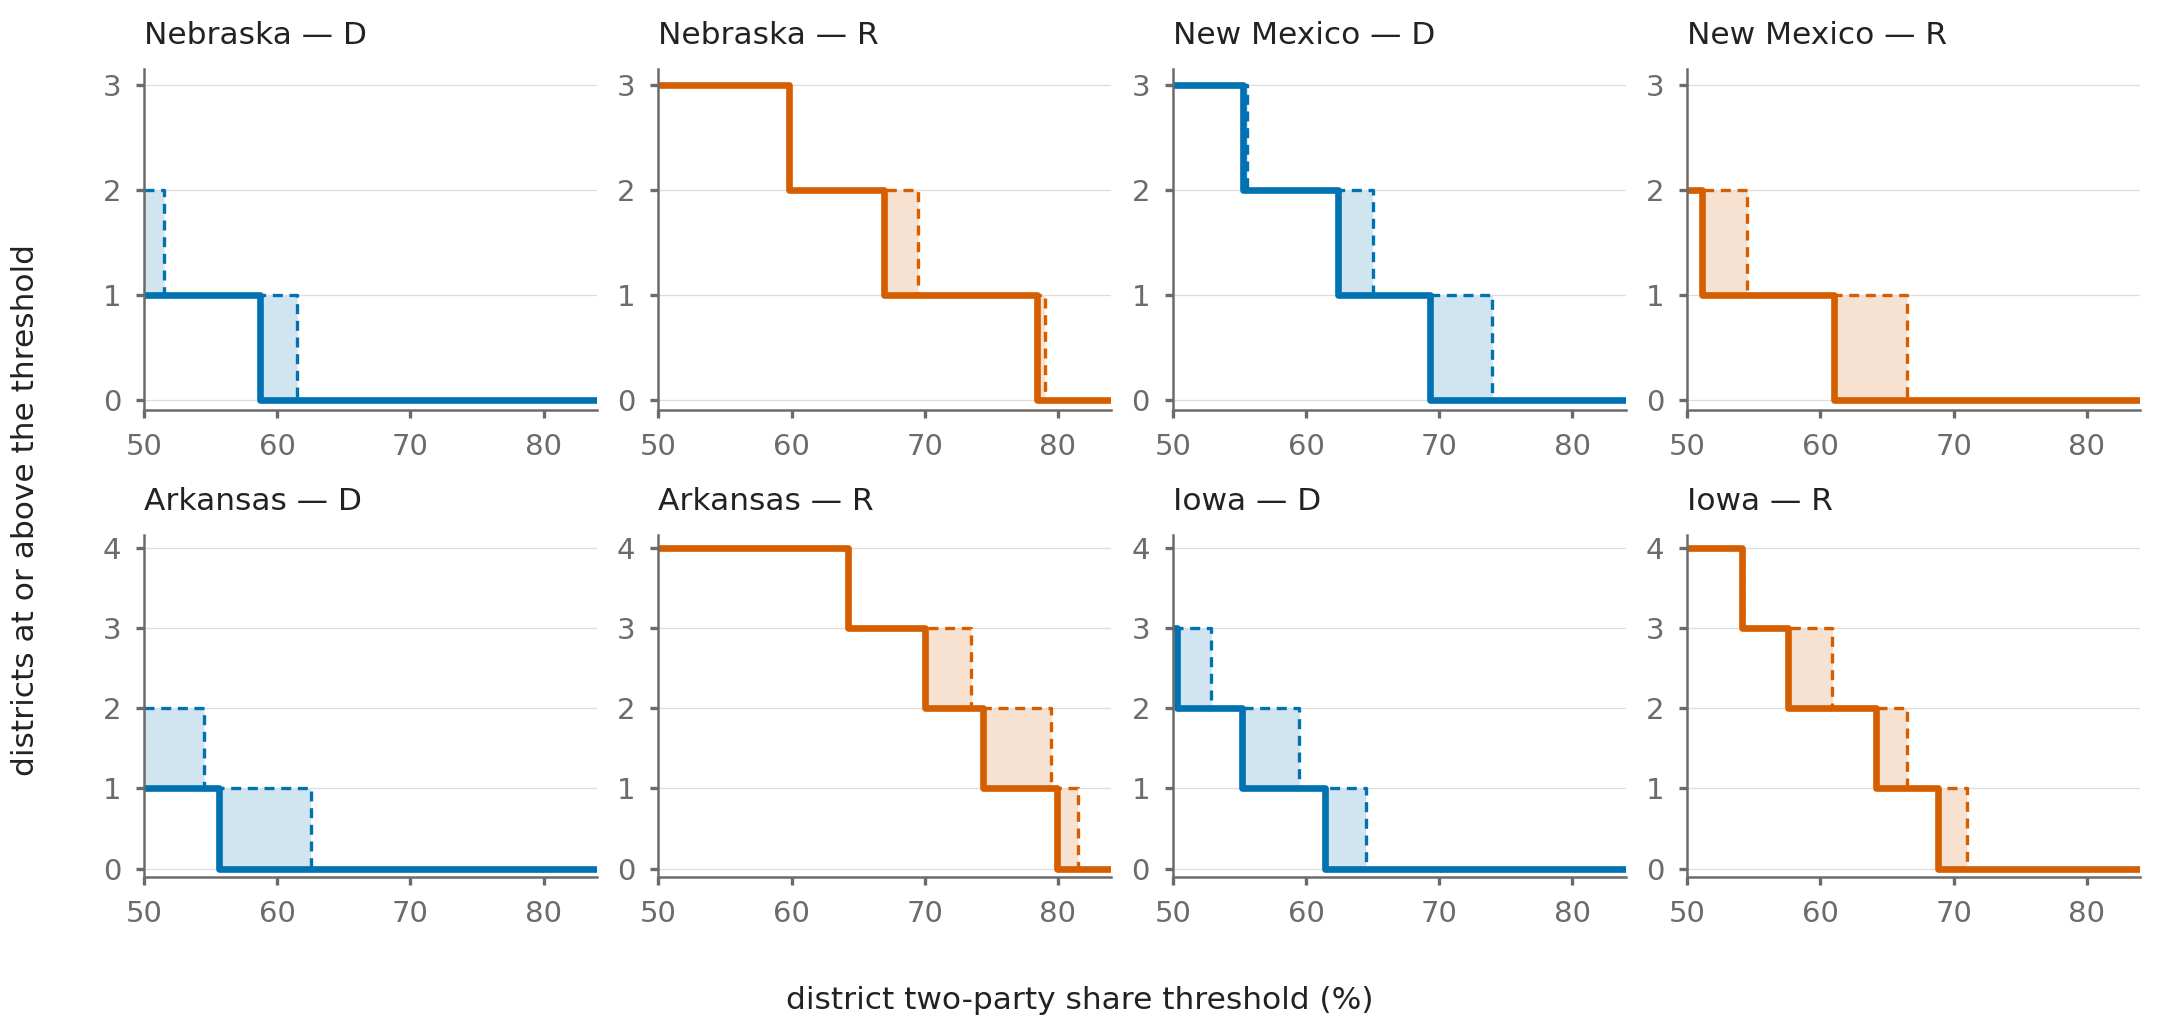
\includegraphics[width=\linewidth]{figs/frontier_k34a.png}\\[4pt]
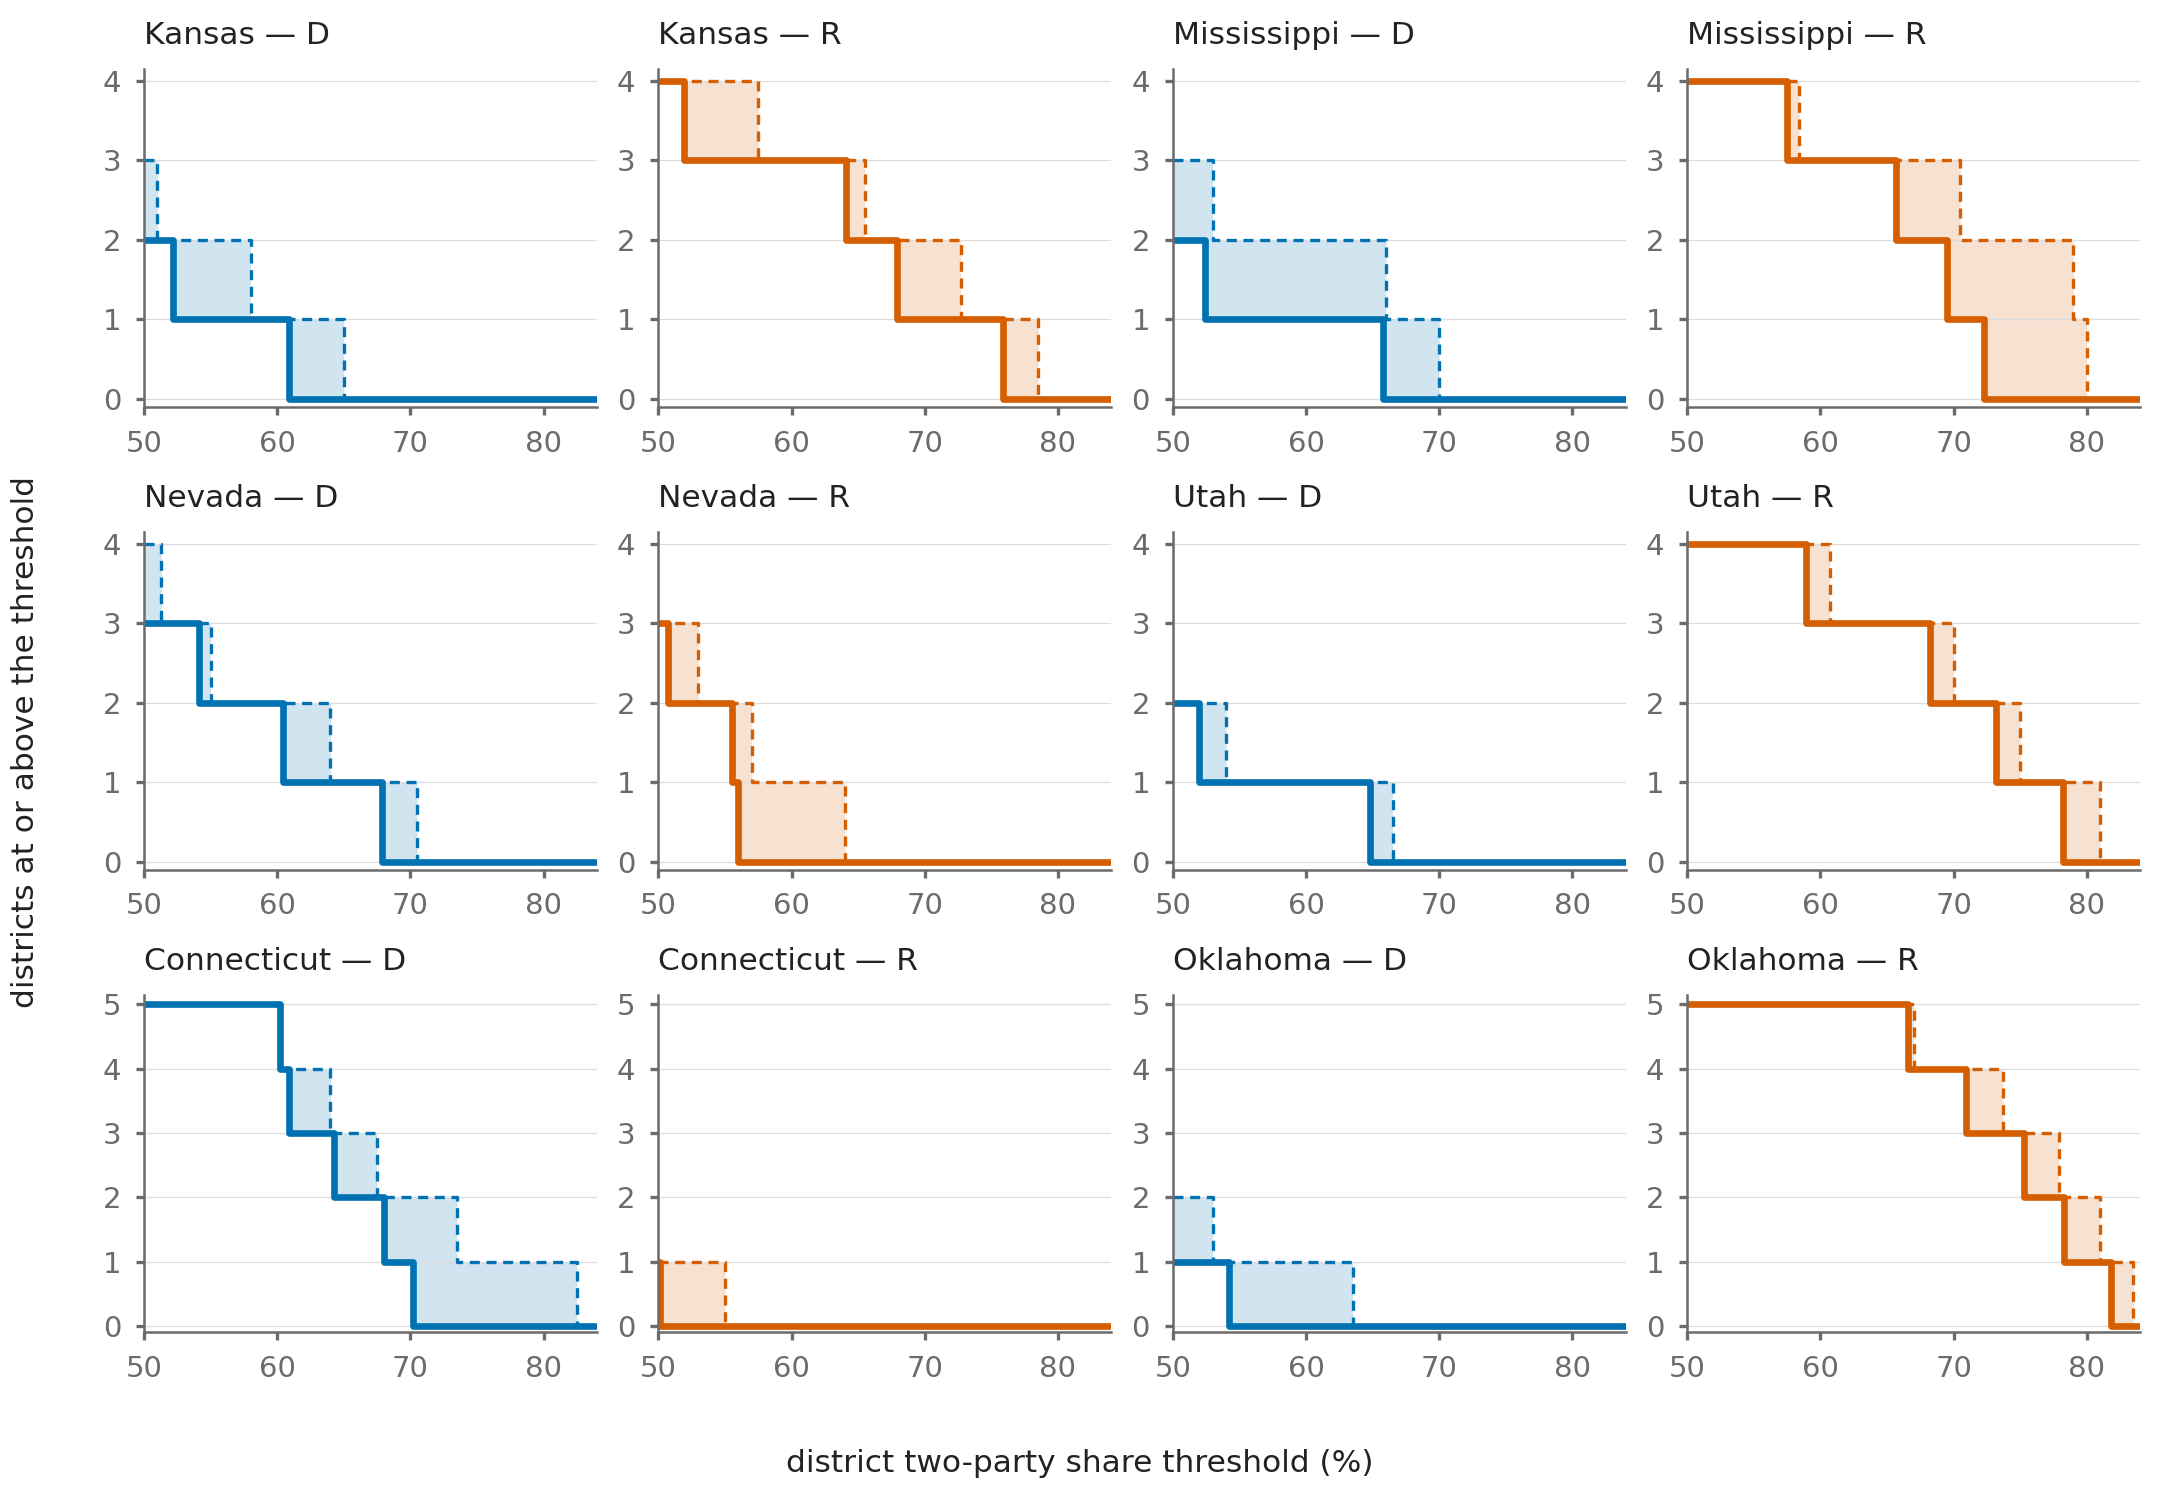
\includegraphics[width=\linewidth]{figs/frontier_k345b.png}
\caption{As Figure~\ref{fig:frontier2} for the states with three to five districts. Shaded bands mark brackets that remain open after the time limits of Section~\ref{sec:results}.}\label{fig:frontier3}
\end{figure}
